\documentclass{article}
\usepackage{graphicx}
\usepackage{float}
\usepackage{qtree}
\usepackage{sidecap}
\usepackage{fullpage}
\usepackage{listings}
\usepackage{color}
\usepackage{tikz}
\usetikzlibrary{shapes,arrows, matrix, positioning, fit}
\DeclareGraphicsExtensions{.pdf,.png,.jpg}
\graphicspath{ {img/} }

% Java code with lstlisting
\definecolor{dkgreen}{rgb}{0,0.6,0}
\definecolor{gray}{rgb}{0.5,0.5,0.5}
\definecolor{mauve}{rgb}{0.58,0,0.82}

\lstset{frame=tb,
    language=Java,
    aboveskip=3mm,
    belowskip=3mm,
    showstringspaces=false,
    columns=flexible,
    basicstyle={\small\ttfamily},
    numbers=none,
    numberstyle=\tiny\color{gray},
    keywordstyle=\color{blue},
    commentstyle=\color{dkgreen},
    stringstyle=\color{mauve},
    breaklines=true,
    breakatwhitespace=true
    tabsize=3
}

\title{CIS4301 Notes}
\author{Ryan Roden-Corrent}
\date{}

\begin{document}
\setlength\parindent{0pt}
% Tikz general settings
\tikzstyle{decision} = [diamond, draw, fill=blue!20, text width=4.5em,
  text badly centered, node distance=3cm, inner sep=0pt]
\tikzstyle{decision2} = [diamond, double, draw, fill=blue!20, text width=4.5em,
  text badly centered, node distance=3cm, inner sep=0pt]
\tikzstyle{block} = [rectangle, draw, fill=blue!20, text width=5em,
  text centered, minimum height=4em]
\tikzstyle{block2} = [rectangle, draw, double, fill=blue!20, text width=5em,
  text centered, minimum height=4em]
\tikzstyle{line} = [draw, -]
\tikzstyle{arrow} = [draw, -latex']
\tikzstyle{cloud} = [draw, ellipse, fill=red!20, node distance=2.5cm,
  minimum height=2em]
\tikzstyle{circle} = [draw, ellipse, fill=red!20, node distance=1.0cm,
  minimum height=1em]
\maketitle

\section{Functions of a Database}
\begin{itemize}
    \item \textbf{Create} - Add new records
    \item \textbf{Query} - Search for records meeting a description
    \item \textbf{Store} - Hold data in records
    \item \textbf{Durability} - data remains available and uncorrupted (backups)\\
        Example: Oracle provides prompt maintenance if a server you bought from
        them goes down
    \item \textbf{Access} - Manageable permissions. Control who can see/edit
        data
\end{itemize}

\section{History of Databases}
\subsection*{1870s}
Charles Babbage and Ada Lovelace create the difference engine, and later, the
analytic engine (mechanical computers)
\subsection*{1876}
Invention of Dewey Decimal system: a general cataloging system for libraries
that is still in use today.
\subsection*{1962}
Bachman: integrated data store
\begin{itemize}
    \item \textbf{network data model}: a tree with no loops
    \item \textbf{graph data model}: loops allowed
\end{itemize}
models are specific to the data being represented
\subsection*{1960s}
\textbf{Disks} (random access) replace \textbf{tapes} (serial access).
Now one can access data without reading the preceding data.\\
At this time, people interested in databases are mostly programmers.\\
IBM Builds \textbf{IMS} (Information Management System) to track Apollo.\\
\textbf{CODASYL:} Commitee standardizzed network data model

\subsection*{1970s} Edward Codd writes 'A relational model of data for large
shared banks'.  It conflicts with the design of the current most popular
databases.  Eventually, IBM agrees to dedicate a research team to Codd's idea;
this team produces SQUARE

\subsection*{1977}
Another IBM team develops \textbf{Query By Example (QBE)}.\\
A group of CIA employees branch off to found \textbf{Oracle} and create the
first commercial implementation of \textbf{SEQUEL}.\\
\textbf{SEQUEL} stands for \textbf{Structured English Query Language} but is
abbreviated to \textbf{SQL} to avoid a copyright dispute.

\subsection*{1990s}
Research into object oriented database implementations

\subsection*{2000s}
Web Boom: Many services suddenly need to store massive amounts of data.

\section{NOSQL}
\begin{description}
    \item{1970} No SQL - SQL doesn't exist
    \item{1980} SQL invented, standard for databases
    \item{1990} No, SQL - If you want to do database stuff, use SQL
    \item{2000} Not Only SQL - There are other things out there
    \item{2010} No, really, use SQL
\end{description}

\section{Is a filesystem a database?}
\begin{description}
    \item[Create] can create and remove records (touch, rm, mkdir, rmdir)
    \item[Query] can search records (find, windows search bar)
    \item[Store] files can sotre content that can be read back
    \item[Durability] debateable
    \item[Access] issues arise if two sources try to edit the same file
\end{description}
Which of these services are actually part of the filesystem, and which are
really provided by the operating system?

\section{Applications Of Databases}
\begin{description}
    \item[Bank] Store Account information
    \item[Social Media Site] User info, posts, need to find users/posts by query
    \item[Advertising] Store and utilize user data for targeted advertising
    \item[Music Library] Query music by artist, album, or other property
    \item[Employee Records] Name, salary, ect.
\end{description}

\subsection{Early Database Adopters}
Early adopters of database systems were banks, airlines, telecom companies, and
companies interested in tracking employee data.

\subsection{Large Database Users}
\begin{enumerate}
    \item Google/Youtube
    \item NSA
    \item Amazon
    \item Yahoo
    \item Yahoo
    \item Facebook
    \item Sprint
    \item AT\&T
    \item Apple
    \item National Energy Research Scientific Computing (NERSC)
    \item Lexis Nexis
\end{enumerate}

All of these companies keep track of \textbf{user-generated content}

\section{An overview of DMBS}
\textbf{DDL}: Data Definition Language\\
CREATE, ALTER, DROP, TRUNCATE, COMMENT, RENAME\\
\textbf{DML}: Data Manipulation Language\\
SELECT, INSERT, UPDATE, DELETE

\subsection{Flow of a query}
$Query \rightarrow Query Parser \rightarrow Query Plan \rightarrow Query
Preprocessor \rightarrow Query Optimizer \rightarrow Query Plan$\\
SQL is declaritive - say what you want, and an optimal search method is chosen
for you
\subsection{Query Structure}
$f_2(f_1(Table_1, Table_2)), Table_3)$\\
\Tree[.f_2  \textit{Table_3} [.f_1 [\textit{Table_1} \textit{Table_2} ]]]\\
The query optimizer may collapse this\\
$f_3(Table_1, Table_3)$\\
\Tree [.f_3 \textit{Table_1} \textit{Table_3} ]\\
\subsection{Parts of a Database}

\begin{figure}[H]
    \centering
    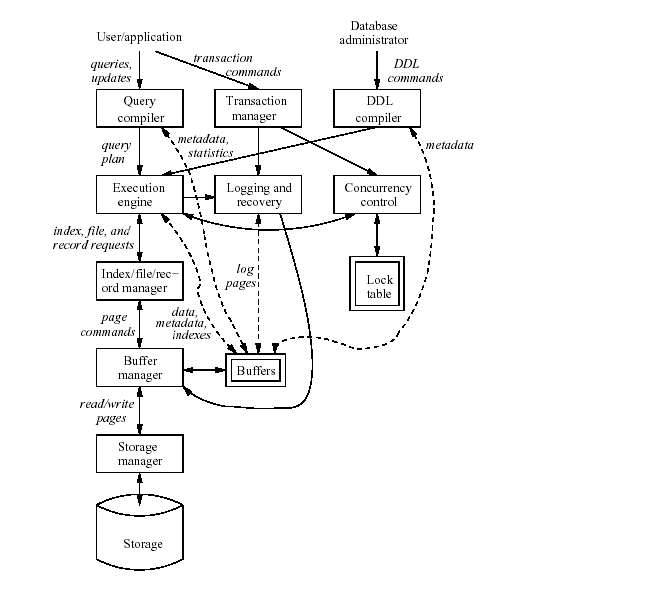
\includegraphics[scale=0.5]{dbms}
    \caption{Database Flow Diagram}
\end{figure}
\begin{description}
    \item[Query Compiler] {Form query}
    \item[Index/File/Record Manager] {Can speed up queries using index}
    \item[Buffer Manager] {Decide whether to cache in RAM (much faster than disk!)}
    \item[Storage Manager] {Provide access to data on disk in \emph{pages}}
    \item[Transaction Manager] {Process transactions (see next section)}
\end{description}

\section{Transactions}
Transactions are operations that must be executed reliably and consistently.
Order is important, and transactions should not interfere with eachother.
In \textbf{multi-threaded} applications, race-conditions and deadlocks can occur
while trying to execute transactions. Deadlock resolution must occur.
Transactions are atomic - they need to happen all at once or not at all.
The transaction manager must initiate \textbf{rollback} (undo) in case of an
error. Transactions are run in isolation from other database operations. 

\subsection{ACID}
\begin{samepage}
\begin{description}
    \item[Atomicity] transaction happens just once or not at all
    \item[Consistency] predictable ordering, same result every time
    \item[Isolation] no interference between transactions 
    \item[Durability] no data missing after transaction
\end{description}
\end{samepage}

\subsection{Transaction Example}
\begin{verbatim}
cg == 1
T_1
BEGIN
1/13 | cg | +5
1/14 | cg | -1
END;
cg == 5

T_2
BEGIN
1/13 | cg | -5
1/13 | cg | +1
END;

End result should be the same regardless of order of execution
T_1; T_2 == 1
T_1; T_2 == 1

\end{verbatim}

\section{Relational Data Model}
\begin{enumerate}
    \item{Physical Model}
    \item{Operations on data}
    \item{Constraints on data}
\end{enumerate}

\subsection{Physical Model Example}
\begin{samepage}
\begin{lstlisting}
public class Animal
{
    public int Eyes;
    public String birthDate;
    public double Weight;

    public void beCute();
}

Animal a = new Animal();
[header][integer][birthDate...][double][beCute]
\end{lstlisting}

Constraints:
\begin{itemize}
    \item{birthDate can't be null}
    \item{Eyes can't be negative}
\end{itemize}
\end{samepage}

\subsection{Relational Model}
Separate data from operations.

\begin{description}
    \item[Relations] {no more than 2}
    \item[Attributes] { order matters, \textbf{atomic} (int,double,String) }
    \item[Tuples]
    \item[Domain]
    \item[Keys] uniquely define attribute instance
\end{description}

\subsection{Relational Model Example}

\begin{figure}[h!]
\begin{tikzpicture}[node distance = 2cm, auto]
  \node [block] (ani) {animal};
  \node [cloud, left of=ani] (weight) {weight};
  \node [cloud, above of=ani] (eyes) {eyes};
  \node [cloud, left of=eyes] (birthday) {birthday};
  \node [decision, right of=ani] (owned) {owned by};
  \node [block, right of=owned, node distance=3cm] (owner) {owner};
  \node [cloud, above of=owner] (ssn) {\underline{ssn}};

  \path [line] (weight) -- (ani);
  \path [line] (birthday) -- (ani);
  \path [line] (eyes) -- (ani);

  \path [line] (ani) -- (owned);
  \path [arrow] (owned) -- (owner);

  \path [line] (ssn) -- (owner);
\end{tikzpicture}
\end{figure}
The underline indicates that \underline{ssn} is the unique key for an owner. As
the set (birthday, weight, eyes) uniquely identifies an animal, they do not need
to be underlined.

\begin{lstlisting}

Animal(eyes:integer, birthDate:String, weight:double)
(0001, 2, "November 2", 12.0) //cannot have 2 of these, must be unique
(0002, 3, "November 2", 12.0)

//don't have to store entire animal, could just store certain columns
var a[] = [2,3]  
\end{lstlisting}

\subsection{Thinking with Relational Models}
Don't think about how data will be stored, just how it will be used.\\
Entity Relational Model:
\begin{description}
    \item[ Entity/Sets ]
    \item[ Relationships ]
    \item[ Attributes ]
\end{description}

\subsection{Constraints}
\begin{description}
    \item[many-many]
    \item[one-one]
    \item[one-many/many-one]: a pet only has one owner, an owner may have many
        pets
\end{description}

\begin{figure}[H]
  \centering
  \begin{minipage}{.5\textwidth}
    \centering
    \caption{one-one relation}
    \begin{tikzpicture}[node distance = 0cm, auto]
      \node [circle] (a1) { };
      \node [circle, below of=a1] (a2) { };
      \node [circle, below of=a2] (a3) { };
      \node [circle, below of=a3] (a4) { };

      \node [circle, below right= 0.5cm and 2cm of a1] (b1) { };
      \node [circle, below of=b1] (b2) { };
      \node [circle, below of=b2] (b3) { };

      \path [line] (a1) -- (b1);
      \path [line] (a2) -- (b2);
      \path [line] (a3) -- (b3);

      \node [draw=blue, thick, 
      fit=(a1) (a2) (a3) (a4) (b1) (b2) (b3)] {};
    \end{tikzpicture}
  \end{minipage}%
  \begin{minipage}{.5\textwidth}
    \centering
    \caption{many-many relation}
    \begin{tikzpicture}[node distance = 0cm, auto]
      \node [circle] (a1) { };
      \node [circle, below of=a1] (a2) { };
      \node [circle, below of=a2] (a3) { };
      \node [circle, below of=a3] (a4) { };

      \node [circle, below right= 0.5cm and 2cm of a1] (b1) { };
      \node [circle, below of=b1] (b2) { };
      \node [circle, below of=b2] (b3) { };

      \path [line] (a1) -- (b1);
      \path [line] (a1) -- (b2);
      \path [line] (a2) -- (b2);
      \path [line] (a4) -- (b3);
      \path [line] (a3) -- (b3);

      \node [draw=blue, thick, 
      fit=(a1) (a2) (a3) (a4) (b1) (b2) (b3)] {};
    \end{tikzpicture}
  \end{minipage}%
\end{figure}

\section{Data Models}
\subsection{Important Aspects}
\begin{description}
  \item[Efficient Access]{}
  \item[Efficient Modification]{}
  \item[Programmer Productivity]{}
\end{description}

\subsection{JAVA Data Access example}
\begin{lstlisting}
class Animal {}

Animal kizzy = new Animal();
kizzy.getEyeCount();

Vector<Animals> cats = new Vector<>();
cats.get(3).talk();

// Options for serialization
//serialize as binary 
byte[]catBytes = cats.serialize();

try {
  http.push(catBytes);
}

//serialize as XML 
<cats>
  <cat name='kizzy'>
    <name>kizzy</name>
  </cat>
</cat>

//serialize as JSON
cats = {
  cat = [ { name: 'kizzy', eyes: 2}, { name: 'garfield' } ]
}

//later
Vector<Cats> v = cats.unserialize(bytes);

//search for a specific element
for (Cats c : v) {
  if (c.name = 'kizzy')
    //found it
}

\end{lstlisting}

\begin{description}
  \item[Efficient Access]{Get from disk and serialize}
  \item[Efficient Modification]{Get from disk, deserialize, modify, reserialize}
  \item[Programmer Productivity]{}
\end{description}

\subsection{SQL Data Access example}
\begin{samepage}
  \begin{lstlisting}[language=SQL]
CREATE DATABASE cats;
CREATE TABLE cats (
  name VARCHAR,
  eyes integer
);
INSERT cats VALUES ('kizzy', '2');

SELECT name
FROM cats
WHERE name = 'kizzy'
\end{lstlisting}
\end{samepage}

\section{Entity Relationship (ER) Models}
\subsection{Example ER Model}

\begin{figure}[h!]
\begin{tikzpicture}[node distance = 2cm, auto]
  \node [block2] (logins) {logins};
  \node [cloud, left of=ani] (billing) {billing};
  \node [cloud, above of=ani] (name) {\underline{name}};
  \node [decision2, right of=ani] (at) {at};
  \node [block, right of=owned, node distance=3cm] (host) {host};
  \node [cloud, above of=host] (hostname) {\underline{name}};
  \node [cloud, right of=host] (url) {url};

  \path [line] (billing) -- (logins);
  \path [line] (name) -- (logins);

  \path [line] (logins) -- (at);
  \path [arrow] (at) -- (host);

  \path [line] (hostname) -- (host);
  \path [line] (url) -- (host);
\end{tikzpicture}
\end{figure}

Host is a \textbf{strong entity} (can exist on its own)\\
Login is a \textbf{weak entity} (cannot exist without Host)\\
\begin{description}
  \item[Host] uniquely identified by name
  \item[name] underlined - key for Host (must be unique)
  \item[URL]
  \item[At] Circular arrow - maps to a single Host, cannot exist without it
  \item[Logins] A login requires a Host
  \item[name] underlined - key for name (must be unique)
  \item[Host]
\end{description}

\subsection{Schema Format}
\begin{itemize}
  \item{Host(\underline{name}, URL)}
  \item{Logins(\underline{name}, \underline{host.name}), billing}
\end{itemize}

\end{document}
